To define the network architecture of the solution to be created, some aspects must be remembered. One is that there are various communication technologies that may be used, as presented previously in Market Research. Other important aspect to keep in mind is that this solution implements both Smart Street Lighting and Smart Parking, through the use of street lampposts. So, these must have parking spots nearby, in order to allow full use of the Smart Parking feature. In order to fulfill the city needs in street lighting, this lack of flexibility demands a creation of a similar solution, without the Smart Parking feature, that won't be approached in this project.

The data stream in the network will be very low since each lamppost will only communicate notifications on it's state. That is, if the lamp is light up, if it was detected a malfunction with the lamp, if it was detected an available parking space. Furthermore, since the street lampposts may be far apart from the gateway, there is the need to use a long range communication technology, to maximize the number of nodes connected to a single gateway.

In figure \ref{fig:LoRa_Range}, one can see that LoRa is ideal for applications that transmit small chunks of data with low bit rates. Data can be transmitted at a longer range compared to technologies like Wi-Fi, Bluetooth, ZigBee or cellular communication technologies like Sigfox or \ac{lte-m}, as presented previously. These features make LoRa well suited for sensors and actuators that operate in low power mode. LoRa can be operated on the \ac{ism} license free sub-gigahertz bands, for example, 915~MHz, 868~MHz, and 433~MHz. It also can be operated on 2,4~GHz to achieve higher data rates compared to sub-gigahertz bands, at the cost of range. \cite{lora_lorawan}

\begin{figure}[ht]
	\centering
	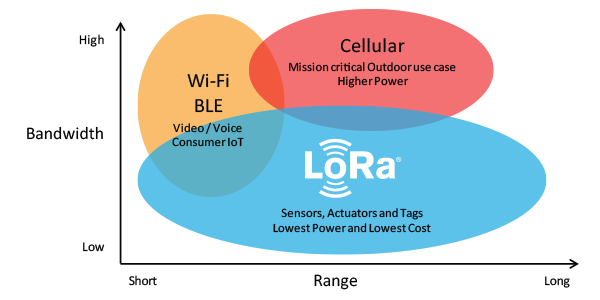
\includegraphics[width=0.69\textwidth]{/03system_overview/LoRa_Range}
	\caption{Communication technologies range vs bandwidth.}
	\label{fig:LoRa_Range}
\end{figure}

\clearpage
With that in mind, one can identify LoRa as a proper communication technology to use in this network. 

In figure \ref{fig:network_arch} one can see the network architecture diagram. This is a star topology, in which the gateway relay messages between each local system (lamppost) and a central network server, the remote system. This wireless communication takes advantage of the Long Range characteristics of the LoRa physical layer, allowing a single-hop link between the local system and the gateway. All communication modes are capable of bi-directional communication, and there is support for multicast addressing groups. The gateway is connected to the internet in order to store new information about the network in the remote system.

\begin{figure}[ht]
	\centering
	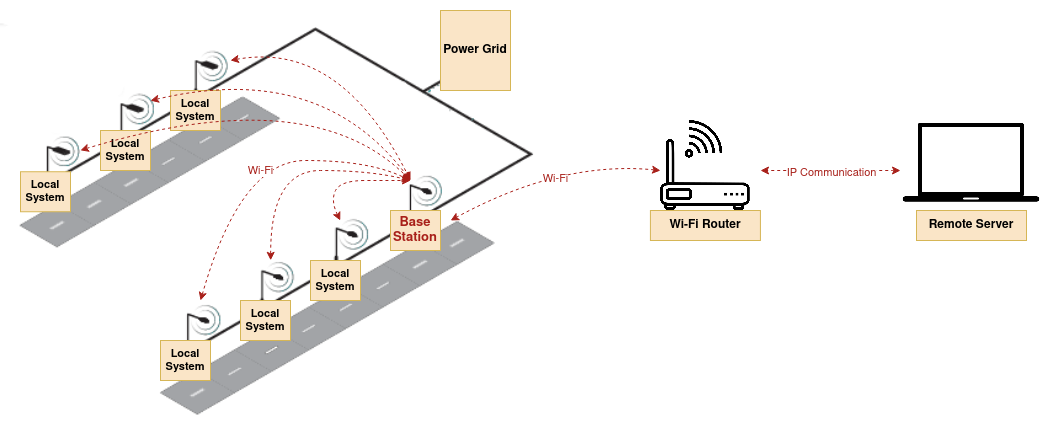
\includegraphics[width=1\textwidth]{/03system_overview/network_arch}
	\caption{Network architecture.}
	\label{fig:network_arch}
\end{figure}
%\clearpage

LoRa end-devices serve different applications and have different requirements, that's why there are device classes, as one can see in figure \ref{fig:lora_device_classes}.

\begin{figure}[H]
	\centering
	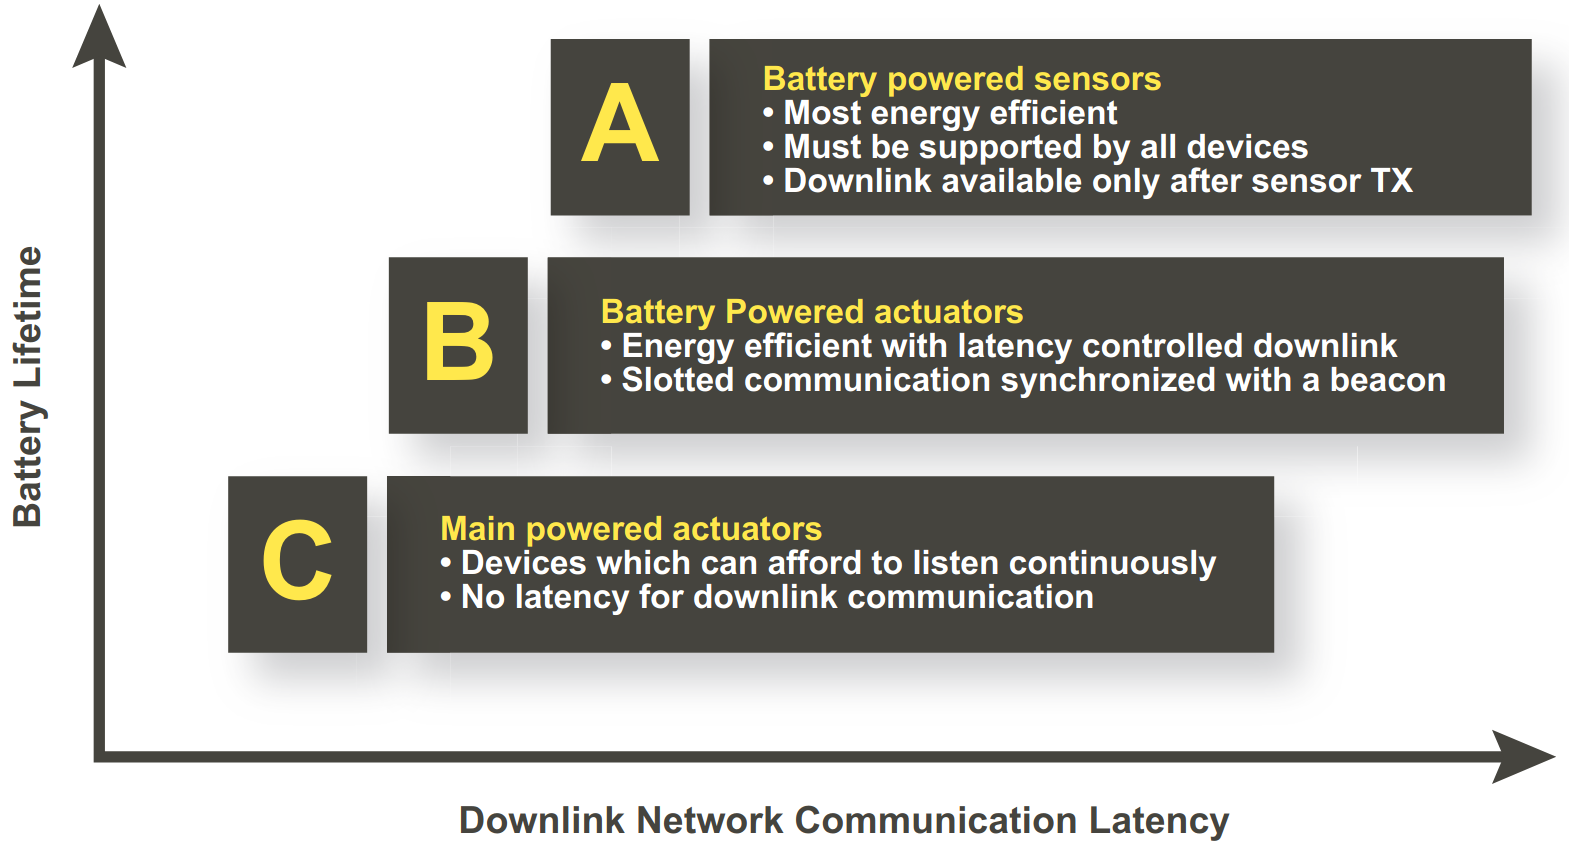
\includegraphics[width=0.7\textwidth]{/03system_overview/LoRa-DeviceClasses}
	\caption{LoRa device classes.}
	\label{fig:lora_device_classes}
\end{figure}

Knowing that street lampposts have main power, from the power grid, one can classify the network nodes as class C. End-devices of class C are bi-directional end-devices with maximal receive slots, has they have almost continuously open receive windows, only closed when transmitting. That way, the downlink communication latency may be very low. \cite{what_is_lorawan}

LoRa provides long range communication, as LoRaWAN gateways can transmit and receive signals over a distance of more than 10 kilometers in rural areas and up to 3 kilometers in dense urban areas. It uses license free spectrum, so one doesn't have to pay expensive frequency spectrum license fees to deploy a LoRaWAN network. It is low cost, since it is a minimal infrastructure, low-cost end nodes and open source software. 

To determine the maximum number of nodes that can be connected to a single gateway, one needs to evaluate gateway specifications, more specifically, the number of packets it can support. For instance, if there is a gateway supporting 1 million packets per day, and if the application sends 10 packet per hour, or 240 packets per day, then, more than 4000 nodes can be handled by that gateway. This is just a rough approximation, since it depends on the packet format/length, on the time needed for the node to send that packet, on the time needed for the gateway to process that packet, and many other constraints that at this point aren't fully identified.



